\let\textcircled=\pgftextcircled
\chapter{Contributions}
\label{chap:contrib}

\initial{C}\textit{e chapitre présente notre contribution à la résolution du problème ci-dessus présenté. Nous montrons au travers de cette contribution comment nous répondons aux questions Q1 et Q2 énoncées au chapitre précédent.}

\minitoc

\newpage  
\section{Contributions sur le plan architectural}

\subsection{Design actuel du PML}

\subsubsection{Architecture}
L'architecture actuelle duu PML se présente telle que sur la figure \ref{fig:pml_actuel} suivante :
\begin{figure}[H]
    \centering
    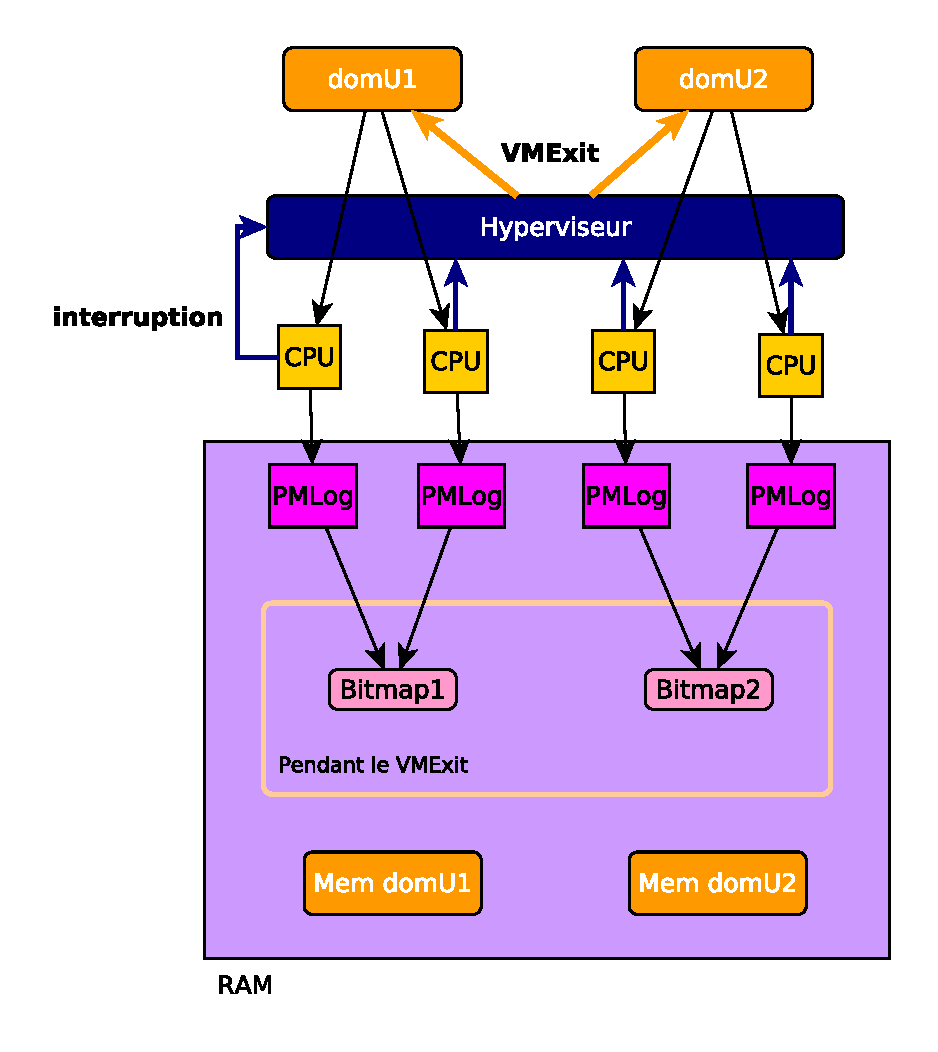
\includegraphics[scale=.8]{chapters/3/fig3/PMLactual3}
    \caption{Architecture actuelle du PML}
    \label{fig:pml_actuel}
\end{figure}

Considérons deux VMs \textit{domU1} et \textit{domU2} \footnote{domU pour \textit{domain Unprivileged} en opposition au dom0 qui est l'OS hôte avec tous les droits et accès.} comme présentées sur la figure précédente. Chacune de ces VMs s'exécute sur des processeurs virtuels, \ac{vCPU}, rattachés à des processeurs physiques (\acs{CPU}).\\
Lorsqu'une VM est créée, si le PML est activée pour celle-ci, alors dans sa structure de contrôle \ac{VMCS}, l'adresse et l'index du PML sont initialisés (voir \ref{subsubsection:description_pml}). Pendant son exécution :

\begin{enumerate}[label=\textbf{(\roman*)}]
    \item Le CPU logue en mémoire centrale, dans le \textit{pml\_log}, les adresses de toute page que la VM modifie. A chaque page modifiée, le CPU ajoute une entrée dans le log.
    \item Lorsque le \textit{pml\_log} est plein, i.e. lorsqu'il contient déjà 512 adresses loguées, le CPU sur lequel s'exécute la VM génère une exception \textit{pml buffer full} qui est prise en main par l'hyperviseur.
    \item L'hyperviseur capture cette exception et en impute le coup à la VM sous la forme d'un \textit{VMExit}.
    \item Pendant ce \textit{VMExit} :
    
        \begin{itemize}
            \item Etant donné que la VM ne s'exécute plus, aucune adresse supplémentaire n'est loguée.
            \item Le CPU parcourt la bitmap associée à la VM et met à jour le bit correspondant à chaque gPA. Si on veut savoir quelles pages ont été modifiées, il faudrait parcourir cette bitmap et retrouver les adresses correspondant chaque bit.
            \item Et enfin le \textit{pml\_log} est vidé, i.e. la valeur de son index (\textit{PML index}) est remis à 511 \footnote{L'index du PML va de 511 à 0.}. 
        \end{itemize}
    
    \item Une fois que le \textit{pml\_log} est vidé, la VM résume son exécution et le processus recommence.
\end{enumerate}

\noindent Le PML a été introduit pour améliorer :
\begin{itemize}
    \item La migration des machines virtuelles
    \item Le checkpointing \cite{checkpointing} des machines virtuelles
    \item Les opérations liées au working set des machines virtuelles (collecte des statistiques de \textit{working set}, estimation du \textit{working set}, etc.)
\end{itemize}

\noindent L'architecture telle que présentée s'est déjà avérée adéquate pour les deux premiers points, mais en ce qui concerne le \textit{working set}, elle présente certaines limites.

\subsubsection{Limites de l'architecture actuelle}
\label{subsubsection:limites_pml_actuel}
Nous présentons ici les principales contraintes auxquelles nous avons fait face avec l'architecture actuelle du PML, et qui l'empêchent d'être efficace à 100\% pour l'estimation du WSS.

\paragraph{\textbullet\ \textbf{Limite 1 : Le VMExit lors de l'interruption \textit{pml buffer full} ne devrait pas être géré par le CPU sur lequel s'exécute la VM dont on estime le WSS}}
\par\noindent
\par\noindent Lorsque le buffer du \textit{pml\_log} est plein, le CPU génère un \textit{VMExit} qui stoppe l'exécution de la VM qui utilise actuellement le CPU en question, cette VM est celle dont le WSS est calculé. Un changement de contexte est donc effectué pour que l'hyperviseur prenne ne main cette interruption. Or les transitions \footnote{Passage du mode non-root au mode root. (Voir sous-section \ref{subsubsection:intel_vtx})} liées aux \textit{VMExits} sont connus pour introduire des coûts significatifs dans la VM \cite{overhead_VMExit}. Ainsi accroître le nombre de \textit{VMExits} sur une VM du fait de l'évaluation de son \textit{working set} est inacceptable pour le client car cette opération n'est bénéfique que pour le propriétaire du DC qui veut optimiser l'utilisation de ses ressources et économiser de l'argent. En effet, le client a payé pour une quantité de ressources (ici le temps CPU) qui doit être allouée à sa VM. En générant des \textit{VMExits} supplémentaires, le design actuel du PML réduit le temps CPU réservé par le client. En outre, le temps pris par l'hyperviseur pour capturer cette exception accroît cet impact.\\
Cette limite n'est pas un problème ni pour la migration ni pour le checkpointing car il a été prouvé que réduire le temps CPU durant ces opérations a pour but de les accélérer \cite{cpu_time_migration}.

\paragraph{\textbullet\ \textbf{Limite 2 : La taille du \textit{pml\_log} est très petite (4KB)}}
\par\noindent
\par\noindent La taille du buffer \textit{pml\_log} a été fixée par Intel à 4KB, pouvant ainsi contenir uniquement 512 gPAs. Cette taille est très petite quand on regarde la plupart des applications de nos jours. La conséquence de ceci est la proportion significative des \textit{VMExits} dus à l'interruption \textit{pml buffer full}, impactant ainsi la VM cible comme présenté à la limite 1.\\
Pour les mêmes raisons que celles présentées à la limite 1, ce problème n'est un obstacle ni pour la migration ni pour le checkpointing.

\paragraph{\textbullet\ \textbf{Limite 3 : Le PML ne devrait pas loguer uniquement les adresses des pages modifiées}}
\par\noindent
\par\noindent Actuellement, le mécanisme du PML n'enregistre que les pages dont le bit \textit{dirty} passe de 0 à 1, i.e. les pages qui sont modifiées. Or le \textit{working set} d'une VM inclue toutes les pages qu'elle utilise, à la fois les pages modifiées et accédées. Et pour l'instant le PML passe à côté de ces pages auxquelles la VM accède sans les modifier, et donc néglige une bonne partie du \textit{working set}, surtout dans le cas de charges de travail de lecture.\\
Une fois de plus, ceci n'est pas une préoccupation dans le cadre de la migration ni du checkpointing, car pour ces opérations, juste les pages modifiées sont traquées.

\paragraph{\textbullet\ \textbf{Limite 4 : Le PML ne devrait pas loguer les adresses des pages de la table de pages}}
\par\noindent
\par\noindent En cas de \textit{TLB miss}, le processeur doit aller chercher en mémoire centrale l'adresse physique correspondant au gPA à l'origine du défaut de page. Ceci implique une translation gPA --> hPA, et donc un parcours de l'EPT comme présenté sur la figure \ref{fig:parcours_2D} à la sous-section \ref{subsubsection:nested_paging}. Comme nous le montre cette figure, pendant la translation d'adresses il y a quatre pages intermédiaires qui seront modifiées et donc quatre \textit{\acl{gPA}s} qui seront loguées dans le \textit{pml\_log} en plus de l'adresse initiale à l'origine du défaut de page. Donc pour un gPA à loguer en cas de \textit{TLB miss}, on a quatre adresses superflues qui sont également enregistrer, ce qui remplit inutilement le \textit{pml\_log}, et donc accroît le nombre d'interruptions dues à l'événement \textit{pml buffer full}.\\
Ceci n'est pas un problème pour les opérations de migration ou de checkpointing, car pour celles-ci toute mise à jour d'une table de pages doit être enregistrée, y compris les tables de pages des VMs (par exemple pour la retransmission dans le cas d'une migration en direct). 

\paragraph{\textbullet\ \textbf{Limite 5 : Le PML devrait tenir compte de la chaleur\cite{pages_chaudes} des pages dans son mécanisme}}
\par\noindent
\par\noindent En effet, l'estimation du WSS a besoin de connaître la chaleur (le nombre de fois où la page est utilisée) d'une page afin d'être sûr que celle-ci fait bien partie du \textit{working set}. Or pour l'instant, le matériel n'enregistre une page que lorsque son bit \textit{dirty} passe de 0 à 1. Si cette page est de nouveau modifiée dans la suite de l'exécution de la VM, le mécanisme n'en tient plus compte et la page n'est plus loguée étant donné que son bit \textit{dirty} est déjà à 1 et que le matériel ne le remet pas à 0.\\
Ceci n'est pas un problème pour les autres scénarios car pour la migration on a juste besoin de savoir si une page a été modifiée, le nombre de modifications importe peu.

\subsection{Proposition d'un design amélioré pour l'estimation du WSS} 
En fonction des limites évoquées plus haut, nous avons pensé un nouveau design architectural dans le but d'améliorer le mécanisme actuel du PML afin qu'il réponde mieux aux besoins d'estimation du WSS. Ainsi l'architecture que nous proposons se décline à travers les étapes suivantes.

\subsubsection{Redirection des \textit{VMExits} vers le dom0}
\begin{figure}[htp]
    \centering
    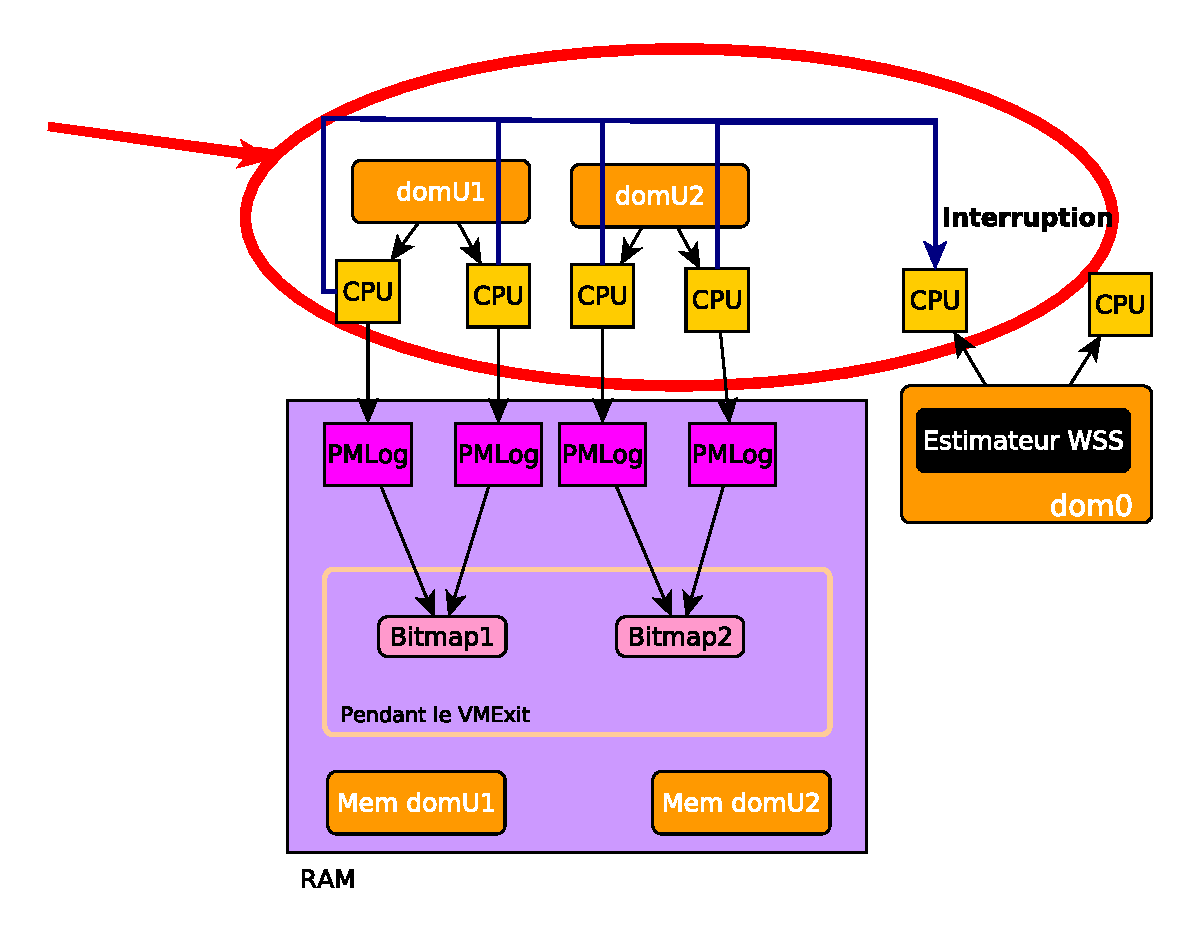
\includegraphics[scale=.8]{chapters/3/fig3/PMLOverview1}
    \caption{Proposition d'une architecture améliorée du PML pour l'estimation du WSS : Redirection des VMExits vers le dom0}
    \label{fig:redirection_vmexit}
\end{figure}
Cette amélioration permettra de palier la limite 1. Comme mentionné dans l'énoncé de cette limite, le coût lié à l'évènement \textit{pml buffer full} ne devrait pas être imputé à la VM (sous le forme d'un \textit{VMExit} comme c'est le cas actuellement).\\
Ainsi, lorsque que le \textit{pml\_log} est plein, nous proposons que le envoie un signal non plus à l'hyperviseur mais au dom0 qui se chargera de traiter cette interruption (Voir figure \ref{fig:redirection_vmexit}).

\subsubsection{Introduction d'une deuxième page de log (\textit{page modification log})}
\begin{figure}[htp]
    \centering
    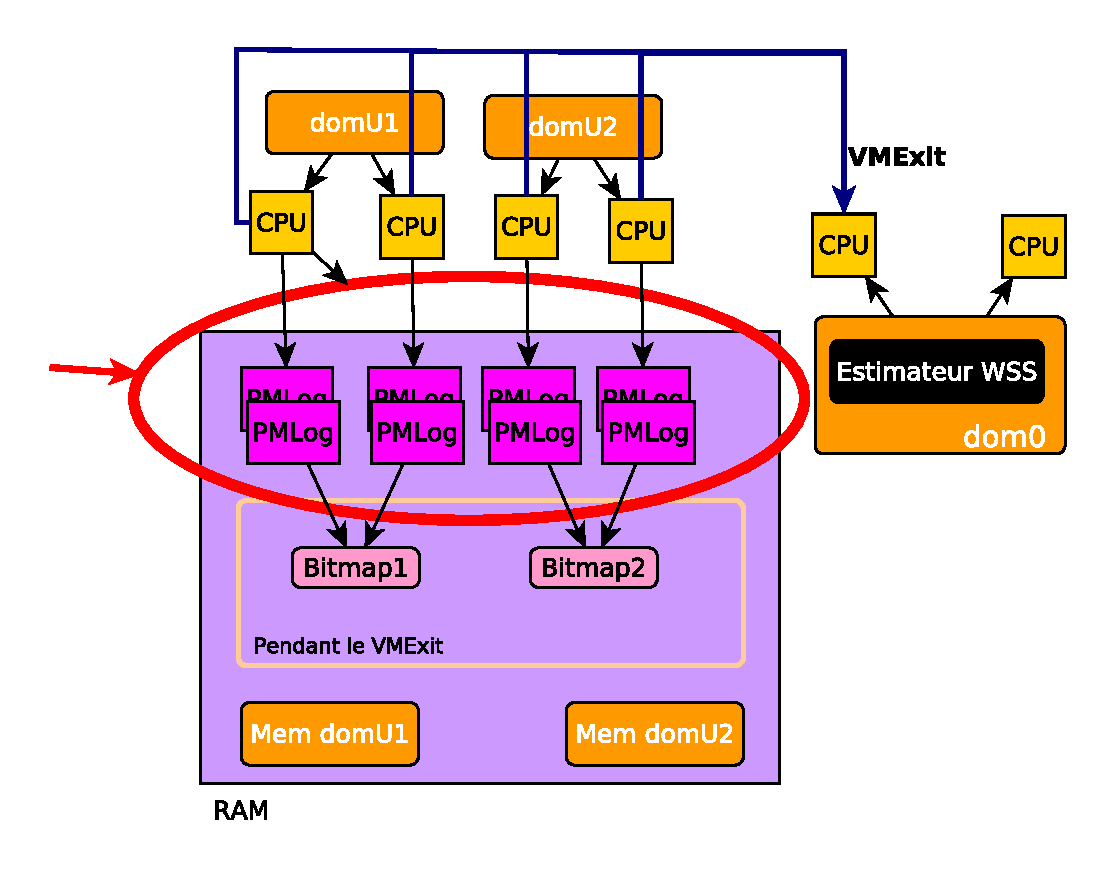
\includegraphics[scale=.8]{chapters/3/fig3/PMLOverview2}
    \caption{Proposition d'une architecture améliorée du PML pour l'estimation du WSS : Introduction d'un deuxième buffer \textit{pml\_log}}
    \label{fig:double_log}
\end{figure}
La figure \ref{fig:double_log} illustre cette deuxième amélioration qui répond à la limite 2, à savoir la taille insuffisante du \textit{page modification log}.\\
En outre, cette nouvelle configuration vient en appoint à la première (redirection des \textit{VMExits} vers le dom0). En effet, lorsque le \textit{pml\_log} sera plein, la VM ne va plus arrêter son exécution, or comme nous l'avons mentionné dans la description du mécanisme actuel, lorsque le \textit{pml\_log} est plein aucune adresse supplémentaire ne peut être loguée dans ce dernier. Ainsi, pour éviter de perdre des adresses nous proposons de rajouter un deuxième \textit{page modification log}, qui pourra continuer d'enregistrer des logs pendant que le premier est vidé. De cette façon, lorsque ce deuxième buffer sera plein, il passera de nouveau la main au premier et ainsi de suite. La VM n'aura donc plus à arrêter son exécution dû à l'évaluation de son WSS, ceci sans empêcher de collecter les statistiques nécessaire à l'estimation.

\subsubsection{Remettre à 0 le bit \textit{dirty} des pages après avoir vidé la page de logs}
Ceci permettra de répondre aux limites 4\&5. En effet, comme nous l'avons expliqué dans la limite 5, une fois que le bit dirty d'une page passe de 0 à 1, le matériel ne le remet pas à 0. Une solution naïve serait de parcourir la table de pages et remettre le bit \textit{dirty} à 0, mais ceci est une opération très couteuse. Nous proposons donc une amélioration qui consisterait à loguer par le matériel l'entrée de la table de pages où la page modifiée a été trouvée. En ayant cette information, il sera aisé de remettre à 0 les bits des pages en évitant les pages de la table de pages (ce qui répond à la limite 4). Pour identifier celles-ci, nous proposons d'utiliser un des bits réservés des tables de pages. Ce bit sera positionné à 1 chaque qu'il y aura un défaut de page concernant une page de la table de pages.

\subsubsection{Modification de la structure de données \textit{bitmap}}
\begin{figure}[htp]
    \centering
    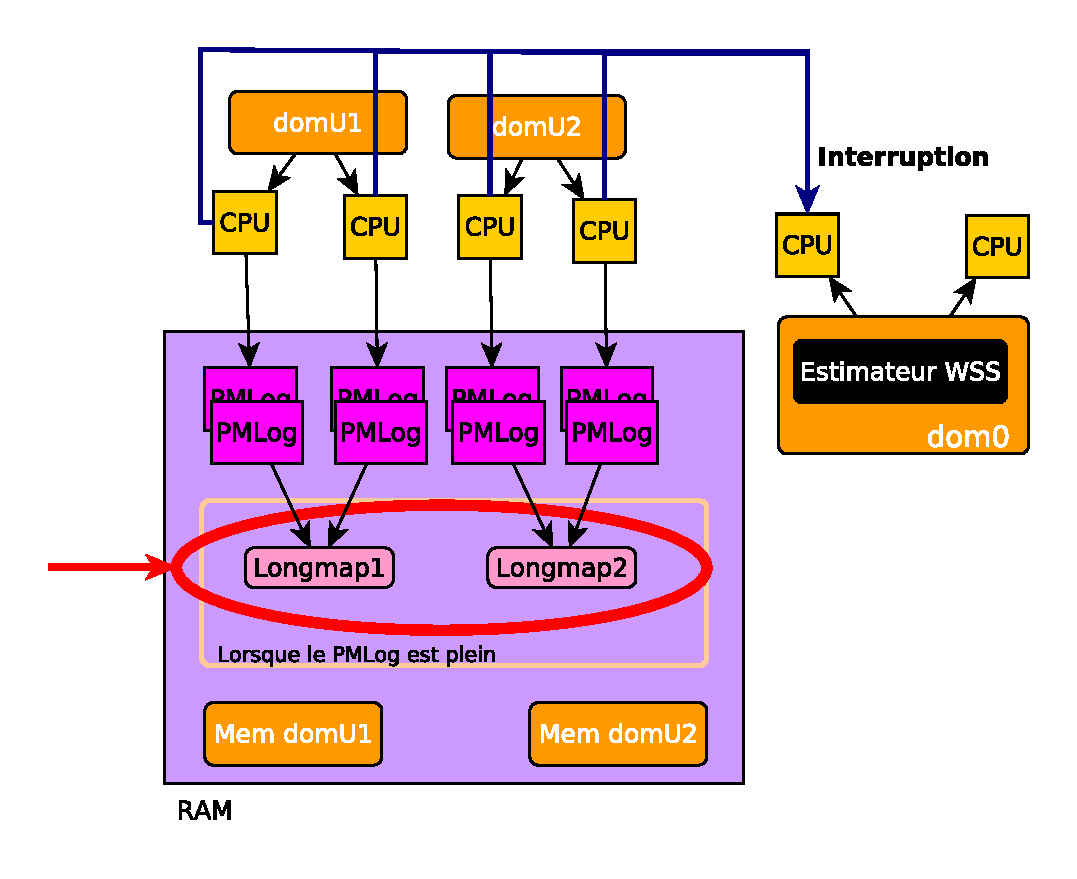
\includegraphics[scale=.8]{chapters/3/fig3/PMLOverview3}
    \caption{Proposition d'une architecture améliorée du PML pour l'estimation du WSS : Modification de la structure de données \textit{bitmap}}
    \label{fig:bitmap}
\end{figure}

\noindent Lorsque le \textit{pml\_log} est plein, avant de réinitialiser son index, les informations qu'il contient doivent être consignées. Actuellement ceci est fait au moyen d'une structure de données appelée \textit{bitmap}  \footnote{Elle est matérialisée par un \textit{radix tree}, un arbre dont chaque a trois noeuds et une feuille terminale. Ce sont les feuilles terminales qui contiennent les bits.}.\\
Chaque VM a en mémoire centrale une \textit{bitmap} qui lui est rattachée. Comme son nom y fait référence, elle est constituée de bits représentant chacune une adresse. Lorsqu'une adresse est dans le \textit{pml\_log}, si le bit y correspondant dans la \textit{bitmap} est à 0, il est mis à 1. De cette façon, il nous est difficile d'avoir plus d'informations sur les données enregistrées telles que les adresses en question ou le nombre de fois où elles ont été modifiées. Et si nous voulions par exemple loguer également les adresses auxquelles la VM a juste accéder, il nous serait impossible de les consigner avec cette \textit{bitmap} dans sa structure actuelle. D'où les limites 3\&5 auxquelles cette modification vient remédier.\\
Nous proposons de modifier l'actuelle \textit{bitmap} de sorte que ses feuilles terminales puissent contenir les informations suivantes :
\begin{itemize}
    \item Les gPAs loguées dans le \textit{pml\_log} : ainsi, lorsque le \textit{pml\_log} sera plein, chacune des adresses qu'il contient sera reportée dans la structure de données.
    \item Un compteur pour chaque gPA : qui représentera le nombre de fois où l'adresse a été modifiée ou accédée. Ainsi, à chaque événement \textit{pml buffer full}, le compteur de chaque adresse présente dans le \textit{pml\_log} sera incrémentée. Ceci nous permettra de connaître la chaleur des pages.
\end{itemize}

\noindent Ainsi, la structure de données de consolidation des logs ne sera plus constituée de bits mais nombres sous forme de \textit{long} \footnote{Le type long, comme integer, ou double.}, d'où la nouvelle appellation \textit{longmap} comme sur la figure \ref{fig:bitmap}.

\section{Algorithmique d'estimation}
\label{section:contrib_algo}
\begin{figure}[H]
    \centering
    \includegraphics[scale=.5]{chapters/3/fig3/courbe_wss_1}
    \caption{Variation de la taille de logs en fonction du temps}
    \label{fig:courbe_wss_cst}
\end{figure}
Avec le mécanisme de PML, l'algorithme consiste à collecter les logs de la VM, et connaissant les adresses des pages qu'elle utilise, déterminer la quantité de mémoire active dont elle a effectivement besoin. Le besoin qui se pose, est de savoir le temps pendant lequel il faut collecter. Soit la courbe \ref{fig:courbe_wss_cst} représentant une variation de la taille de logs en fonction du temps. Lorsqu'on commence à observer une constance dans les logs : 
\begin{itemize}
    \item On arrête la collecte et on estime la taille du \textit{working set} en fonction du nombre d'adresses collectées. La taille d'une page étant de $4Ko$, si on a collecté $n$ adresses, alors on estime le WSS à $M = n*4 Ko$.
    \item On applique l'estimation faite à la VM et pour en être sûr on observe son comportement sur une certaine période.
    \item Si on observe trop de swap ou de défauts de page, alors on effectue de nouveau la collecte et on adapte l'estimation en fonction des observations précédentes.
\end{itemize}

\noindent Seulement la plus part des applications n'ont pas une activité constante.

\begin{figure}[H]
    \centering
    \includegraphics[scale=.5]{chapters/3/fig3/courbe_wss_2}
    \caption{Variation de la taille de logs en fonction du temps}
    \label{fig:courbe_wss_var}
\end{figure}

\noindent Le \textit{working set} de la VM peut être très variable (comme sur la figure \ref{fig:courbe_wss_var}) ou même périodique. Dans la majeure partie des cas, des algorithmes de \textit{machine learning} seront nécessaires pour apprendre le comportement de la VM et savoir quand et comment ajuster sa mémoire.

\noindent Sur la figure \ref{fig:courbe_wss_var}, en se basant sur l'algorithme naïf présenté ci-haut, on arrêterait la collecte à $t1$ et on estimerait le WSS de la VM à $wss1$, ce qui est loin d'être sa valeur exacte. Et en réajustant la VM à cette quantité de mémoire, on la mettrait dans un état de souffrance (la VM sera compressée ce qui conduira à trop de swaps et de défauts de pages).

\section{Avantages de la solution proposée}
Nous avons vu dans le chapitre précédent que toute solution d'estimation du WSS devait répondre à deux questions : 
\begin{itemize}
    \item \textbf{(Q1) : comment observer la VM et collecter les informations sur son \break activité?}\\
    La description du mécanisme du PML répond à cette question. Ici, c'est la matériel lui même qui se charge de collecter pour nous les informations sur l'activité mémoire de la VM, en traquant et les pages utilisées par la VM et en consignant les adresses de celles-ci dans le \textit{pml\_log}. Ce qui rend donc notre solution totalement \textbf{transparente} du point de vue de la VM, i.e. \textbf{non intrusive et non active}.\\
    Actuellement, le coût facturé à la VM concerne l'ensemble des \textit{VMExits} qui lui sont imposés lorsque le \textit{pml\_log} est plein. La solution architecturale que nous proposons vient palier cette limite en redirigeant ces interruptions vers le dom0, donc \textbf{aucune surcharge n'est imposée ni à la VM ni à l'hyperviseur}.
    
    \item \textbf{(Q2) : comment estimer le \textit{working set} de la VM à partir des données collectées?}\\
    Une fois que l'on connaît toutes les pages utilisées par la VM, il nous suffit de les compter et connaissant la taille \footnote{Elle peut dépendre de l'architecture de la machine hôte.} d'une page, il n'y a plus qu'à effectuer le calcul présenté à la section \ref{section:contrib_algo} précédente.\\
    Etant donné que c'est le matériel lui-même qui se charge de récupérer les adresses des pages utilisées par la VM, on peut être sûr qu'aucune adresse ne sera manquée, et donc de la précision de l'estimation. Pour l'instant, cette précision de calcul ne peut être vérifiée car il faudrait d'abord que la nouvelle architecture soit mise sur pied.
\end{itemize}